\subsection{Слой представления}
Для разработки слоя представления была выбрана технология Java Server Pages.
Покажем скриншоты всех имеющихся JSP страниц.
	\begin{figure}[H]
		\centering
		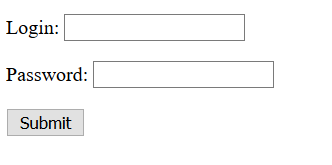
\includegraphics[width=0.5\textwidth]{../materials/Logon.png}
		\caption{Пример страницы авторизации \textit{index.jsp}}
		\label{fig:logon}
	\end{figure}
	\begin{figure}[H]
		\centering
		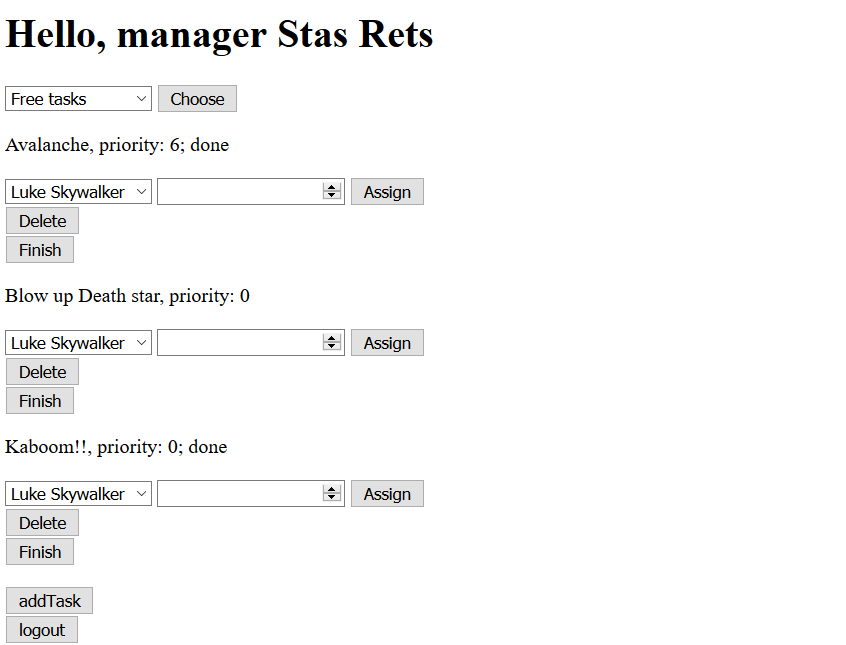
\includegraphics[width=0.8\textwidth]{../materials/Manager.png}
		\caption{Главная страница менеджера \textit{main.jsp}}
		\label{fig:manager}
	\end{figure}
	\begin{figure}[H]
		\centering
		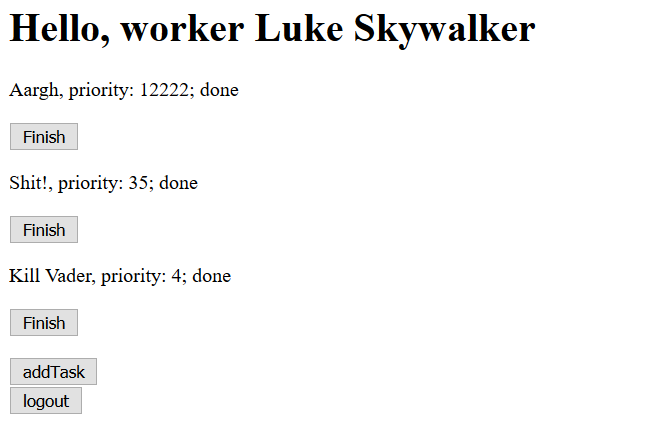
\includegraphics[width=0.8\textwidth]{../materials/Worker.png}
		\caption{Главная страница работника \textit{main.jsp}}
		\label{fig:worker}
	\end{figure}
	\begin{figure}[H]
	\centering
	\includegraphics[width=0.5\textwidth]{../materials/addTask.png}
	\caption{Добавление задачи \textit{addTask.jsp}}
	\label{fig:addTask}
	\end{figure}